\chapter{Computational Definitions and Grammar}

\todo{Needs massive refactor and redux}

Programming languages are the grammar and syntax a computer presents to a user.
This project is fundamentally exploratory in nature and seeks to generate
understanding of geometric relationships using the intersection of
mathematical and computational rigor. 


The REPL (Read-Eval-Print-Loop) allows interactive
evaluation of Julia code. It is highly useful for exploration and testing of
ideas in the language.
Blocks starting with "\texttt{julia>}" represent input and the preceding
line represents output of the evaluated line.

\subsection{History}
Julia is a programming language first released in early 2012 by a group of
developers from MIT. The language targets technical computing by providing a
dynamic type system with near-native code performance. This is accomplished by
using three concepts: a Just-In-Time (JIT) compiler to target the LLVM framework,
a multiple dispatch system, and code specialization.\cite{bezanson2012julia}
\cite{Bezanson_Edelman_Karpinski_Shah_2014}
The syntactical style is similar to MATLAB and Python.
The language implementation and many libraries are available under the
permissive MIT license.\footnote{\url{http://opensource.org/licenses/MIT}}

Benchmarks have shown the language can consistently perform within a factor of
two of native C and FORTRAN code.\footnote{\url{http://julialang.org/benchmarks}}
This is enticing for a solid modeling application and for numerical analysis,
as the code abstraction can grow organically without performance penalty.
In fact, the authors of Julia call this balance a solution to the 
``two language problem". The problem is encountered when abstraction in a
high-level language will disproportionately affect performance unless
implemented in a low-level language. In the next sections we will compare
the expressibility and performance to other languages.

\subsection{Comparisons}

Many languages are as fast as Julia but sacrifice expressibility.
In Figure \ref{fig:juliabench} we can see some comparisons to other programming
languages. This was developed by the Julia core team, and illustrates that
Julia is highly competitive in performance. Again, these results stem from
the compiler and language design. In Figure \ref{fig:juliaexpr} we can see
these results normalized against code length. The Julia code is quite short,
yet consistently achieves good performance.
Much of this comes down to the innovated type and function system.\cite{Chen2014} We will
discuss these more in depth later.

\begin{figure}[h!]
  \centering
    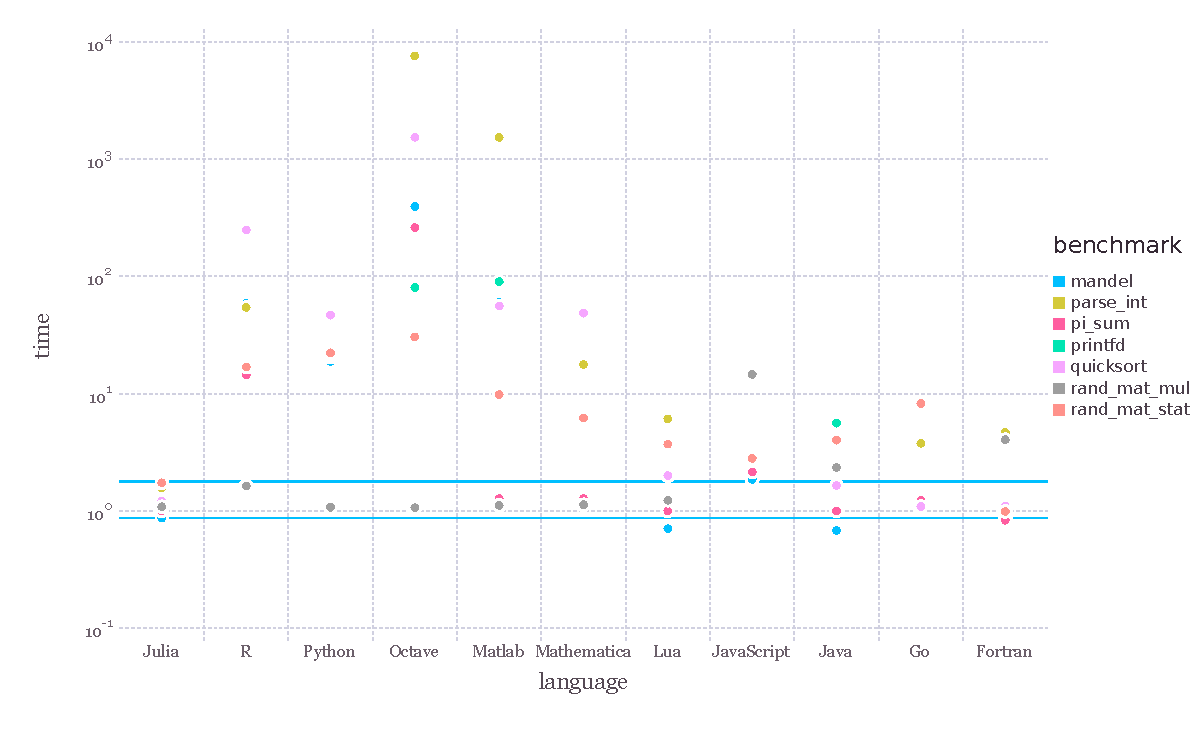
\includegraphics[width=1.0\textwidth]{img/juliabench.pdf}
  \caption{A comparison of programming languages and performance.}
  \label{fig:juliabench}
\end{figure}

\begin{figure}[h!]
  \centering
    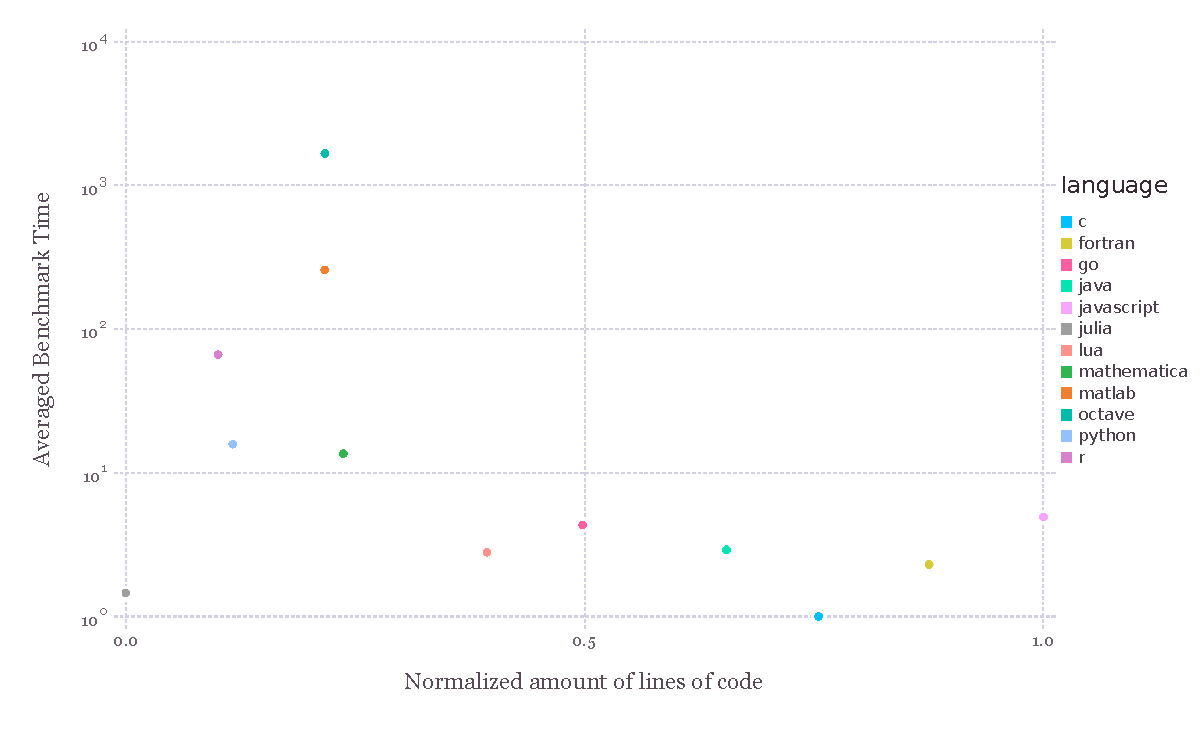
\includegraphics[width=1.0\textwidth]{img/expressability.pdf}
  \caption{The results in Figure \ref{fig:juliabench} normalized for code length. (Courtesy of Simon Danish)}
  \label{fig:juliaexpr}
\end{figure}


In 1972 Alan Kay introduced the terms
"class" and "object", to describe a coupling of data and functionality.\footnote{\url{http://gagne.homedns.org/~tgagne/contrib/EarlyHistoryST.html}}
An object is simply and implementation of a class. Computer Scientists
call this "Object Oriented Programming" (OOP).
Languages such as C++, Java, and Python all subscribe to this paradigm.
In Python this looks like the following:
\begin{lstlisting}
class Foo:
    foo1
    foo2
    def add_to_foo1(self, x):
        self.foo1 += x
\end{lstlisting}

This system positively enables specialization of functionality, but due
to the coupling of data with functions it becomes a challenge to extend
functionality. Languages for scientific computing generally avoid the
"traditional" notions
of OOP. In Table \ref{tab:types} we can see a
comparison of type systems used in scientific computing languages. In the next
few sections the implications of multiple dispatch and the relation to OOP
will be developed further.


\begin{figure}[h!]
  \centering
    \caption{A comparison of functions, typing, and dispatch.}
    \begin{tabular}{ l | l l l}
    Language & Type system & Generic functions & Parametric types \\
    \hline
    Julia & dynamic & default & yes \\
    Common Lisp & dynamic & opt-in & yes (but no dispatch) \\
    Dylan & dynamic & default & partial (no dispatch) \\
    Fortress & static & default & yes \\
    \end{tabular}
  \label{tab:types}
\end{figure}


\subsection{Functions}
Julia is an experiment in language design. Much of the advancement
revolves around the representation of data and the execution of functions.
The language is optionally typed, which means function specialization on types
is inferred. We will use it See below:
\begin{lstlisting}
julia> increment(x) = x + 1
increment (generic function with 1 method)

julia> increment(1)
2

julia> increment(1.0)
2.0
\end{lstlisting}
the \texttt{increment} function was defined for any \texttt{x} value. When the
\texttt{1}, an
integer type was passed as an argument, an integer was returned. Likewise
when a floating point, \texttt{1.0} was passed, the floating point
\texttt{2.0} was returned.

Let's see what happens when we try a string:
\begin{lstlisting}
julia> increment("a")
ERROR: MethodError: `+` has no method matching +(::ASCIIString, ::Int64)
Closest candidates are:
  +(::Any, ::Any, ::Any, ::Any...)
  +(::Int64, ::Int64)
  +(::Complex{Bool}, ::Real)
  ...
 in increment at none:1
\end{lstlisting}

The problem is that the \texttt{+} function is not implemented between the
\texttt{ASCIIString} and \texttt{Int64} types.
We need to either implement a \texttt{+} function
which might be ambiguous, or specialize the function for \texttt{ASCIIString}.
A specific implementation is preferrable in this case:
\begin{lstlisting}
julia> function increment(x::ASCIIString)
           ASCIIString([increment(c) for c in x])
       end
increment (generic function with 2 methods)
\end{lstlisting}
The line \texttt{x::ASCIIString} is called a ``type annotation" and
states that \texttt{x} must be a subtype
of \texttt{ASCIIString}. This allows one to control dispatch of functions,
since Julia will default to the \emph{most specific implementation}.
Since\texttt{ASCIIString} is a series of 8 bit characters, we can iterate over the
string and increment each character individually. The \texttt{[]} indicates we are
constructing an array of characters to pass to be passed to the \texttt{ASCIIString}
type constructor. Now we see our example works:
\begin{lstlisting}
julia> increment("abc")
"bcd"
\end{lstlisting}

What was demonstrated here is the concepts of specialization and multiple
dispatch, both are highly coupled topics.
Each function call in Julia is specialized for types if possible.
This means the author only has to write a few sufficently abstract
implementations of functions. If special cases occur multiple functions
with different arity or type signatures can be implmented. Explicitly
this is called multiple dispatch. In practice by the user this looks like
abstracted or generic code.
To the computer, this means choosing the most specific, and
thus performant method. Let's go back to the integer and floating point
example. Below is the LLVM assembly generated for each method:
\begin{lstlisting}
julia> @code_llvm increment(1)

define i64 @julia_increment_21458(i64) { // <return type> <function name>(<arg type>)
top:
  %1 = add i64 %0, 1
  ret i64 %1 // return <return type> <return id>
}

julia> @code_llvm increment(1.0)

define double @julia_increment_21466(double) {
top:
  %1 = fadd double %0, 1.000000e+00
  ret double %1
}
\end{lstlisting}

Note I have annotated the LLVM code so this is understandable. 
The only real similarity is the line count. Each one of these functions are generated by the
Julia compiler at run time.

Many of the concepts used for performance also serve as methods for
expressability. In this case, multiple dispatch used by the compiler for
specialization of functions reveals it self as a way for the user to
specialize over many types.
Revealing the role in which this paradigm allows Julia to achieve high
performance is a matter to be developed in further sections.

\subsection{Types}

\subsubsection{Mutability and data packing}
Types and immutables are containers of data. The primary difference between
the two is the notion of "mutability". Types are mutabile, immutables are 
immutable. What does this mean? Let's break something first:
\begin{lstlisting}
julia> type FooIsMutable
           a
       end

julia> f = FooIsMutable(1)
FooIsMutable(1)

julia> f.a
1

julia> f.a = 2
2

julia> f.a
2

julia> immutable FooIsImmutable
           a
       end

julia> f = FooIsImmutable(1)
FooIsImmutable(1)

julia> f.a
1

julia> f.a = 2
ERROR: type FooIsImmutable is immutable
\end{lstlisting}

What just happened demonstrates the contract defined by mutability. Mutable
objects, which is an instance of a type (i.e. \texttt{f}), can have their fields
(i.e. \texttt{a}) changed. Immutables cannot. The immutable contract helps develop
a notion of functional purity. To the user this means immutables are defined
by their values. Practically this can be of great benefit to
the compiler. For example:
\begin{lstlisting}
julia> a = (1,2,3)
(1,2,3)

julia> b = typeof(a)
Tuple{Int64,Int64,Int64}

julia> isbits(b)
true

julia> a = ([1],[2],[3])
([1],[2],[3])

julia> b = typeof(a)
Tuple{Array{Int64,1},Array{Int64,1},Array{Int64,1}}

julia> isbits(b)
false
\end{lstlisting}

\texttt{isbits} ask the question ``will this type be tightly packed in memory"? A
\texttt{Tuple} is a fixed-length set of linear, ordered, data. It has syntax for
construction with \texttt{()}. In computations we want our data be close together
for fast access. In modern times we call such data "cache friendly", or
"cache localized". Immutability helps us achieve this. Let's look that the
types inside the 3-tuples and see their \texttt{isbits} status:
\begin{lstlisting}
julia> isbits(Array{Int64,1})
false

julia> isbits(Int64)
true
\end{lstlisting}
Why is this the case? We see that \texttt{Int64} is bits, because it is literally
64 bits. In Julia a \texttt{bitstype} behaves similar to an immutable, and is identified
by value. \texttt{Array\{Int,64\}} is a mutable data type that can vary in size.
This means
the \texttt{Tuple} needs to store the arrays as references, in this case a
pointer. When iterating over a data set, such a ``pointer dereferences" (this is
jargon for accessing the data in memory pointed to by a pointer), can be costly.
Modern CPUs accell when data is linearly packed and pointer-free. The
data can be brought into the CPU's memory cache once and computed without
shuffling between cache and RAM.

\subsubsection{Parameters}

\todo{need to demonstrate why this is HUGELY important for performance and expression}

\subsubsection{Macros and Generated Functions}
Julia is a descendant of the Lisp family of programming languages. Lisp
is a portmanteau for "List Processing". The language was designed to address
the new notion of "types", specifically in application to Artificial
Intelligence (AI) problems.\cite{McCarthy_1966} The notion of an "S-Expression"
was introduced in McCarthy's seminal work. These statements use parenthesis
to denote functions and arguments. Below is an an example of S-Expressions
for addition and multiplication.

\begin{lstlisting}
> (+ 1 1)
2

> (* 3 4)
12
\end{lstlisting}

This syntax is noted for it's mathematical purity.
However it can be a syntactic difficulty for many.
Most of the current popular programming languages
use variants of ALGOL syntax, which is noted for being more readable.
\cite{Hoare}
Julia also uses ALGOL syntax, but is lowered to S-Expressions. This enables
many of the mathematically pure relations we seek to achieve.
In addition S-Expressions are highly conducive to source transforms.
This develops a notion of "Homoiconicity", where the representation of
program structure is similar to the syntax. In Julia we use this property
to make "macros" which enable source code to be transformed based on
structure before compilation.

Generated functions perform a similar function as macros, but at the function
level. They enable source code to be procedurally generated based on types.
Surveys of Computer Science literature show that such a concept is new.
\todo{More on generated functions. Not sure if they should even be mentioned
since they are usually unnecessary}

\todo{More articulate like Graydon Hoare: \url{http://graydon2.dreamwidth.org/189377.html}}

\subsection{Example}

\cite{Shamos_1999}

